\chapter{Introduction}
\label{ch:Introduction}

\section{Background and Problem Statement}
\label{sec:BackgroundProblemStatement}
In recent years, teledermatology, a branch of telemedicine, has become increasingly popular, especially due to the COVID-19 pandemic. Telemedicine uses telecommunications technology to provide healthcare services remotely, allowing patients to consult with healthcare providers without needing in-person appointments. Teledermatology takes advantage of this technology to diagnose and manage skin conditions remotely. Patients use their mobile devices to take pictures of their skin conditions and send these images to dermatologists for analysis. This process removes the need for face-to-face appointments, making healthcare more accessible and convenient. \par
\vspace{\baselineskip}
\noindent
While teledermatology has many benefits, it heavily depends on the quality of the images that patients submit. Many images are not up to standard due to issues like poor lighting, blurriness, or not clearly showing the skin condition \autocite{TrueImage}. These poor-quality images make it difficult for dermatologists to make accurate diagnoses, leading to a back-and-forth exchange of informations between patient and dermatologist. This process can be time-consuming and frustrating, reducing the overall accuracy of teledermatology. \par
\vspace{\baselineskip}
\noindent
To address this problem, it is very important to improve the quality of images taken by patients. This thesis aims to develop an automated image quality assessment (IQA) techniques that can evaluate the quality of images before they are sent to dermatologists. By making sure that only good-quality images are submitted, the reliability and effectiveness of teledermatology can be greatly improved. \par 
\clearpage
\begin{figure}[ht]
    \centering
    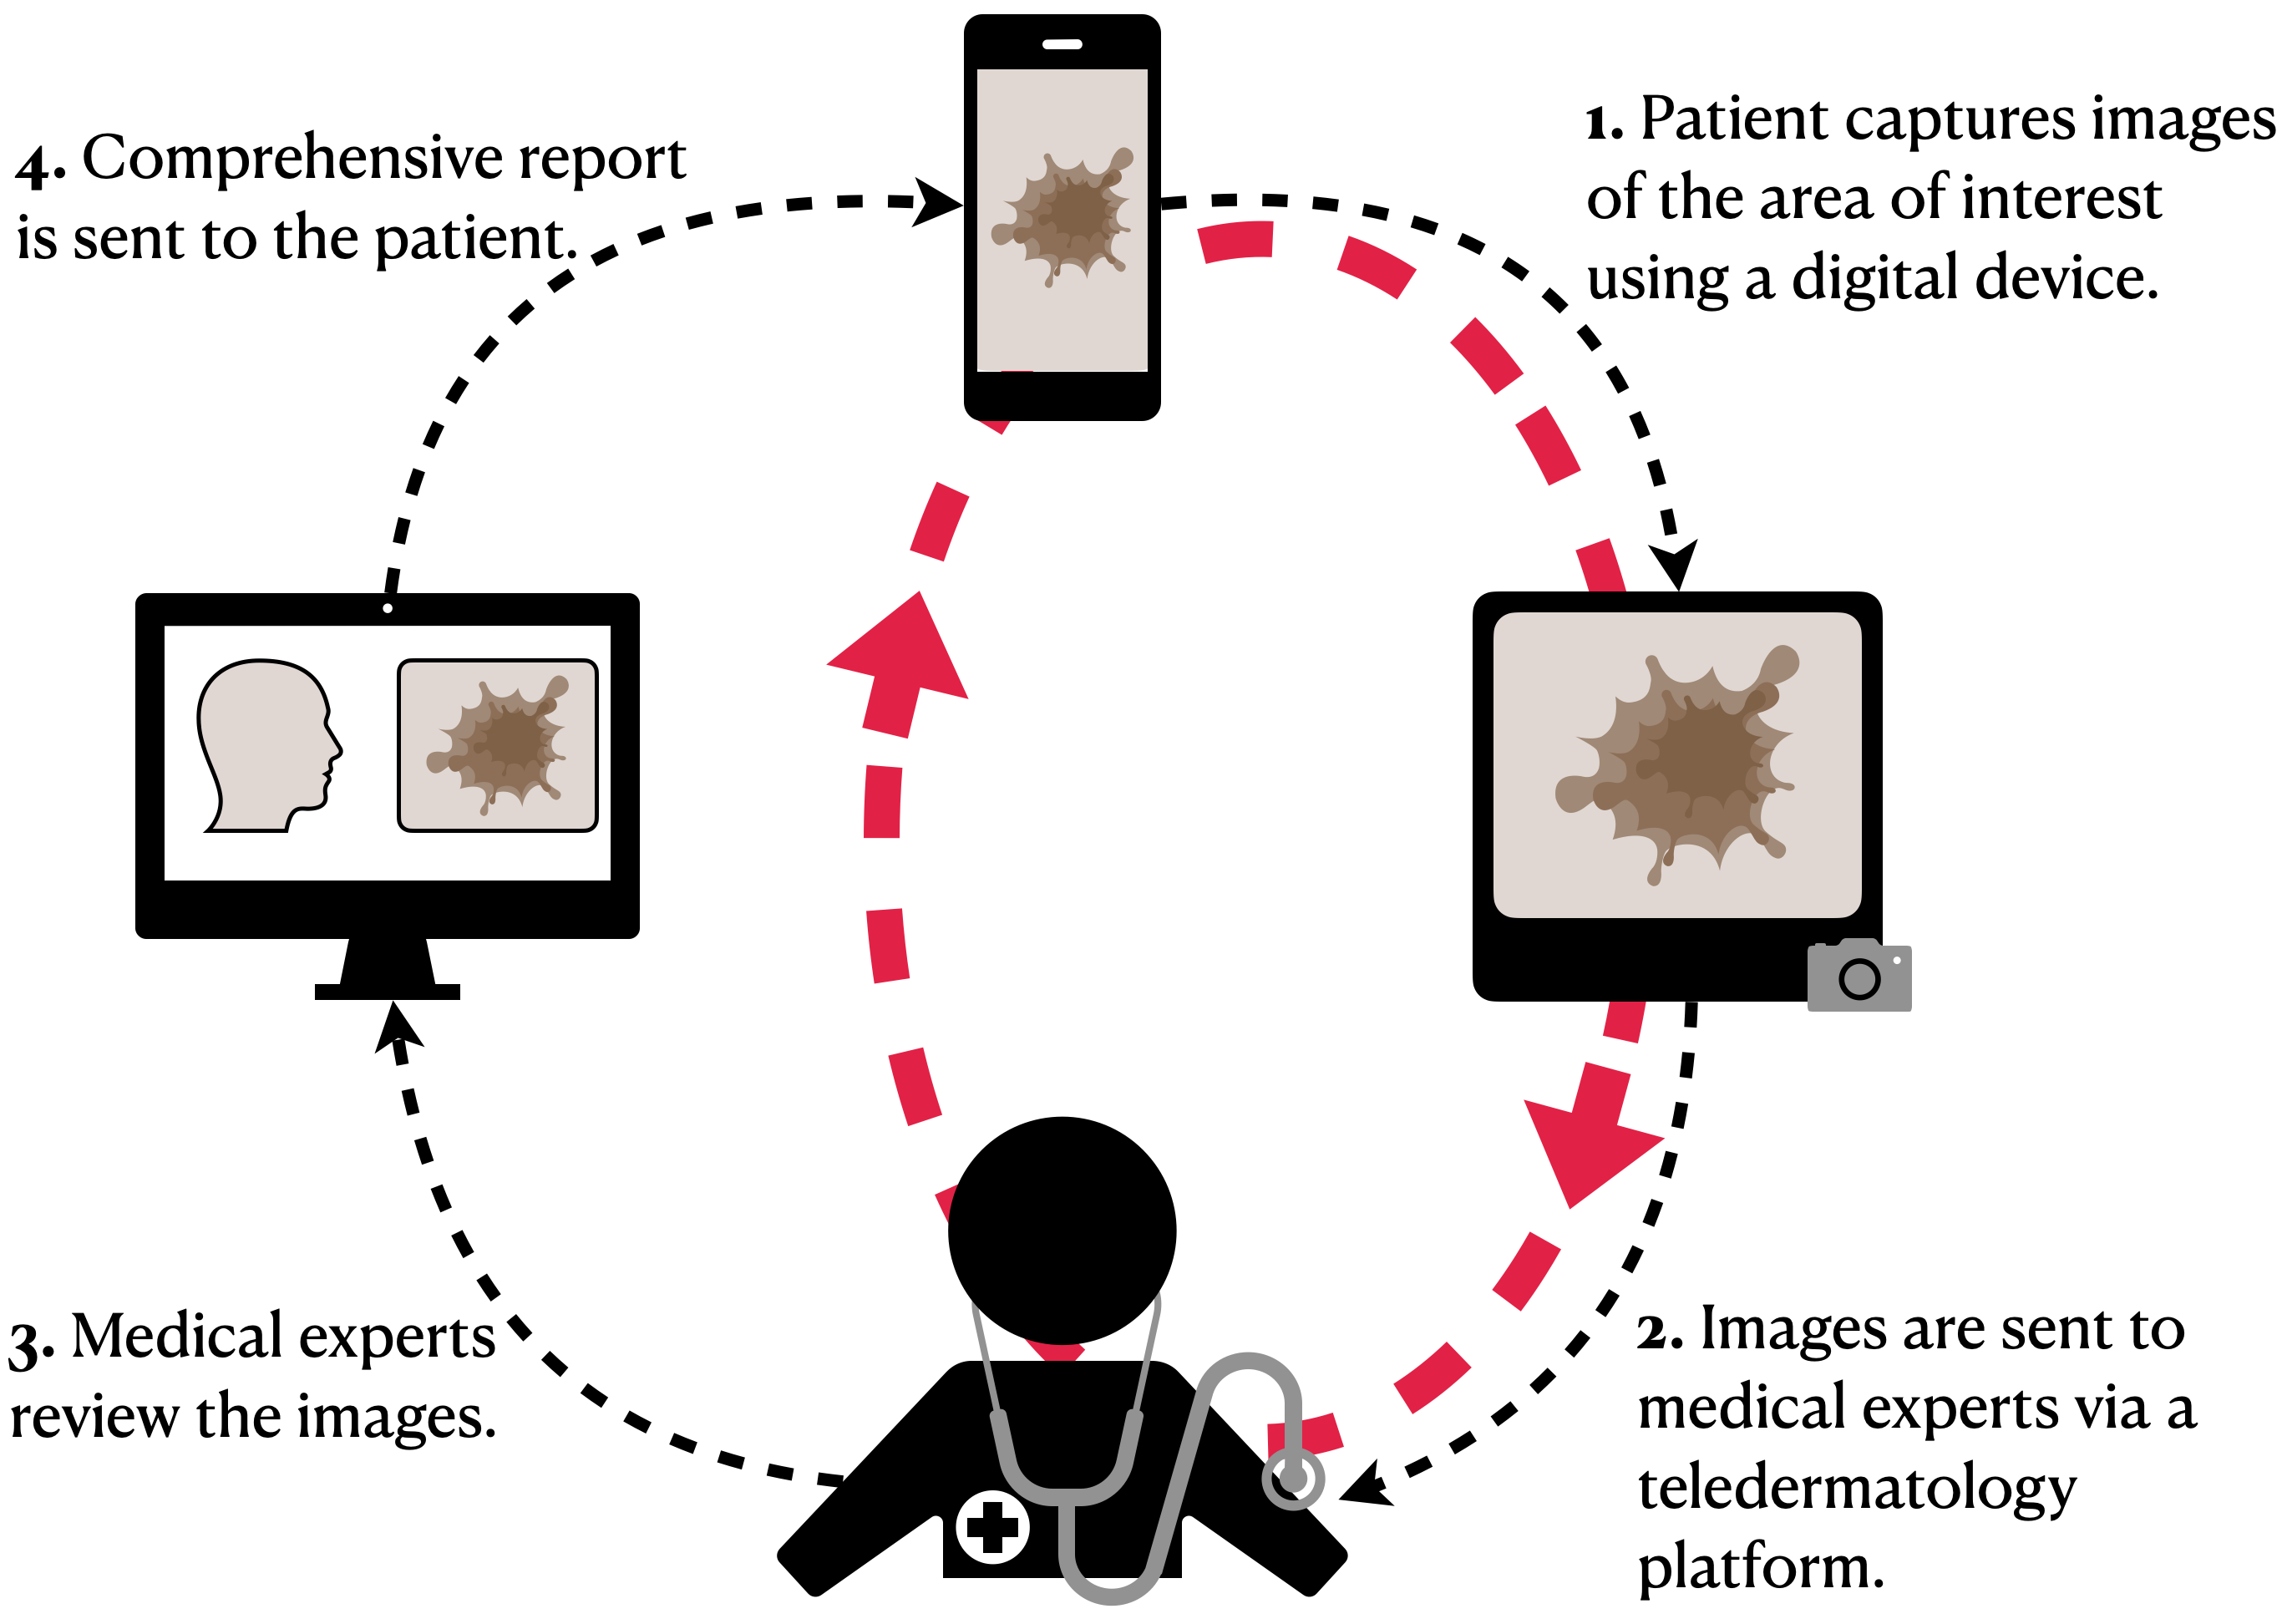
\includegraphics[keepaspectratio,width=13cm]{img/TD_workflow.png}
    \caption{Simplified Teledermatology Consultation Process. The red arrows highlight the back-and-forth exchange due to poor-quality images, which can delay diagnosis and treatment.}
    \label{fig:TD_workflow}
\end{figure}

\section{Objectives of the Thesis}
\label{sec:Objectives}
The primary goal of this thesis is to develop and evaluate automated methods for assessing image quality in teledermatology. The objectives cover several key areas, starting with a detailed review of existing image quality assessment methods. This review will help determine which methods are appropriate for use in the context of teledermatology. The thesis also aims to identify the right dermatology quality criteria, apply selected methods to relevant dermatological images, and create a reproducible repository for future research. \par
\vspace{\baselineskip}
\noindent
The specific objectives of this thesis are as follows:
\begin{itemize}
    \item Conduct a detailed review of existing image quality assessment (IQA) methods, focusing on their use in teledermatology.
    \item  Identify and choose the most appropriate metrics for assessing the quality of dermatological images.
    \item Evaluate the performance of selected image quality metrics on dermatological datasets to determine their effectiveness in assessing image quality.
    \item Create a reproducible repository of tools and methods for assessing image quality in teledermatology.
\end{itemize}
\noindent
Achieving these objectives will greatly improve teledermatology services by providing a reliable way to assess image quality. \par
\clearpage
\section{Organisation of this Thesis}
\label{sec:Structure}
This thesis is structured into seven chapters to provide a clear and systematic exploration of image quality assessment in teledermatology.  \autoref{ch:LiteratureReview} covers the literature review, discussing previous and related works on IQA and teledermatology. \autoref{ch:Methodology} details the methodologies used for the literature review and specific methods for IQA in teledermatology. \autoref{ch:Implementation} describes the experiments conducted, showing the approaches taken and the metrics used. \autoref{ch:ResultsAnalysis} presents the results of the research. \autoref{ch:Discussion} interprets the results, discusses key assumptions and reflects on the findings. Finally, \autoref{ch:Conclusion} summarizes the findings and suggests directions for future research. \par
\vspace{\baselineskip}
\noindent
All figures and tables in this thesis are created by the author unless otherwise referenced. Documents and code relevant to this thesis can be downloaded from the following link: \par \noindent \url{https://github.com/Schoggi-Mimi/bachelor-thesis}. Any code referenced within the thesis is from this repository, with specific paths or modules provided in the footnotes. For simplicity, image quality assessment will be referred to as IQA throughout the document.\par